\newpage
\solutions{Rozstrzygnij, czy}

% Source: https://skm.katowice.pl/pliki/szkice/rejonowe/rozw_rejon_2019.pdf
\begin{problem}{1}
	Rozstrzygnąć, czy istnieją liczby całkowite $x$, $y$, spełniające równanie
	\[
		x^2 - 999y^2 = 1001.
	\]
\end{problem}

\noindent
Wykażemy, że szukane liczby nie istnieją. Przeprowadźmy rozumowanie nie wprost -- weźmy parę~$(x,\; y)$ spełniającą warunki zadania. Skoro zachodzi równość, to w szczególności musi zachodzić przystawanie modulo 3, czyli
\begin{align*}
	x^2 - 999y^2 \equiv 1001 &\pmod{3}, \\
	x^2 \equiv 1001 \equiv 2 &\pmod{3}.
\end{align*}
Jednak kwadrat liczby całkowitej może dawać jedynie reszty $0$ i $1$ z dzielenia przez $3$, co jest sprzeczne z otrzymanym przystawaniem.

\vspace{5px}

% Source: https://dominik-burek.u.matinf.uj.edu.pl/Rabka2017.pdf
\begin{problem}{2}
	Niech $S(\mathcal{X})$ oznacza sumę elementów zbioru $\mathcal{X}$, zaś $S_2(\mathcal{X})$ sumę kwadratów elementów zbioru $\mathcal{X}$. Rozstrzygnąć, czy istnieją takie rozłączne zbiory liczb całkowitych $A$ oraz $B$, które zawierają po $1000$ elementów, że
	\[
		S(A) = S(B) \quad \text{oraz} \quad S_2(A) = S_2(B).
	\]
\end{problem}

\noindent
Wykażemy, że szukane zbiory istnieją.
Rozpatrzmy dowolny zbiór $999$ dodatnich liczb całkowitych~$a_1$, $a_2$, ..., $a_{999}$. Dokładając do niego liczbę
\[
	a_{1000} = - (a_1 + a_2 + ... + a_{999}) 
\]
otrzymamy zbiór liczb niezerowych, których suma wynosi $0$. Rozpatrując zbiór liczb danych jako $b_i = -a_i$ dla wszystkich liczb całkowitych $1 \leqslant i \leqslant 1000$ otrzymamy również zbiór o sumie elementów równej zeru. Wystarczy tylko zauważyć, że
\[
	a_i^2 = (-a_i)^2 = b_i^2,
\]
aby stwierdzić, że sumy kwadratów elementów obu zbiorów są sobie równe. Łatwo też zauważyć, że zbiory te będą rozłączne.

%Source: https://om.mimuw.edu.pl/static/app_main/camps/oboz2019.pdf
\begin{problem}{3}
	Rozstrzygnąć, czy istnieje taka różnowartościowa funkcja $f$ określona na zbiorze liczb całkowitych dodatnich i przyjmująca wartości całkowite nieujemne, że
	\[
		f(mn) = f(m) + f(n)
	\]
	dla dowolnych liczb całkowitych $m$, $n$.
\end{problem}

\noindent
Wykażemy, że żadna funkcja nie spełnia warunków zadania. Załóżmy nie wprost, że $f$ jest takową. Wówczas dla dowolnych dodatnich liczb całkowitych $a$, $k$ mamy
\[
	f(a^k) = f(a) + f(a^{k - 1}) = 2f(a) + f(a^{k - 2}) = ... = k\cdot f(a).
\]
Zauważmy, że
\[
	f(2^{f(3)}) = f(3) \cdot f(2) = f(2)\cdot f(3) = f(3^{f(2)}).
\]
Liczby $2^{f(3)}$ oraz $3^{f(2)}$ mogą być sobie równe wtedy i tylko wtedy, gdy $f(2) = f(3) = 0$. Stąd $f$ przyjmuję tę samą wartość dla dwóch różnych argumentów, co jest sprzeczne z~założeniami zadania.

\vspace{5px}

%Source: https://artofproblemsolving.com/community/c6h1513472p8997062 4 IGO P4 Junior
\begin{problem}{4}
	$P_1,P_2,\ldots,P_{100}$ są $100$ punktami na płaszczyźnie, z których żadne 3 nie leżą na jednej prostej. Dla każdych trzech punktów, nazwijmy trójkąt przez nie tworzony \textit{zegarowym}, jeśli numery wierzchołków są uporządkowane rosnąco zgodnie z ruchem wskazówek zegara. Czy liczba trójkątów zegarowych może wynosić dokładnie $1111$?
\end{problem}

\noindent
Wykażemy, że jest to możliwe. Rozpatrzmy dwie konfiguracje. W jednej punkty są ułożone na okręgu zgodnie z ruchem wskazówek zegara, a w drugiej przeciwnie do niego.
\begin{center}
	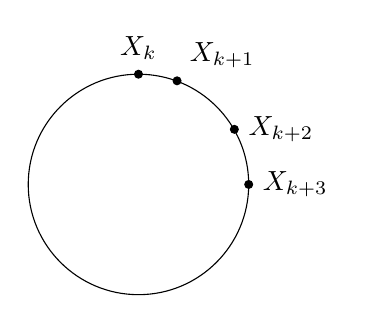
\begin{tikzpicture}[scale=0.7]
		\tikzset{vertex/.style = {shape=circle,draw, inner sep = 1pt, fill=black}}
		\tikzset{edge/.style = {arrowMe=stealth}}


		\node[vertex,label=above:$X_k$] (a) at (0,2) {};
		\node[vertex,label=above right:$X_{k+1}$] (b) at (0.7,1.88) {};
		\node[vertex,label=right:$X_{k+2}$] (c) at (1.74,1) {};
		\node[vertex,label=right:$X_{k+3}$] (d) at (2,0) {};


		\draw (0,0) circle (2);

	\end{tikzpicture}
	\hspace{50px}
	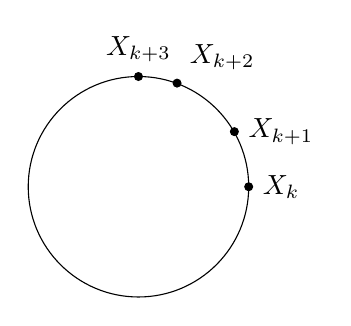
\begin{tikzpicture}[scale=0.7]
		\tikzset{vertex/.style = {shape=circle,draw, inner sep = 1pt, fill=black}}
		\tikzset{edge/.style = {arrowMe=stealth}}

		\node[vertex,label=above:$X_{k + 3}$] (a) at (0,2) {};
		\node[vertex,label=above right:$X_{k+2}$] (b) at (0.7,1.88) {};
		\node[vertex,label=right:$X_{k+1}$] (c) at (1.74,1) {};
		\node[vertex,label=right:$X_{k}$] (d) at (2,0) {};


		\draw (0,0) circle (2);

	\end{tikzpicture}
\end{center}

\noindent
W pierwszej konfiguracji jest ${{{100}\choose{3}} > 1111}$ trójkątów zegarowych, a w drugiej jest ich zero. Wychodząc od pierwszej konfiguracji, zacznijmy przesuwać płynnie punkty tak, aby dojść do konfiguracji drugiej. Najpierw bardzo nieznacznie przesuńmy każdy z punktów, tak, aby zwolnić miejsca, które zajmują. To przekształcenie nie powinno wpłynąć na liczbę trójkątów zegarowych. Następnie przesuńmy punkt $X_1$ na miejsce, które zajmuje on w drugiej konfiguracji. Róbmy to tak, aby nie przejść przez żaden z punktów przecięcia prostych $X_aX_b$ z $X_cX_d$ dla dowolnych liczb naturalnych $1 \leqslant a, b, c, d \leqslant 100$. Analogicznie potem przesuwamy punkt $X_2$, potem $X_3$, ..., aż do $X_{100}$.

\vspace{10px}
\noindent
Zaobserwujmy, że trójkąt $X_aX_bX_c$ zmieni status bycia zegarowym wtedy i tylko wtedy, gdy ruszamy jeden z wierzchołków i przejdziemy nim przez prostą zawierającą pozostały bok. Skoro więc nie założyliśmy, że ruszany punkt przechodzi przez co najwyżej jedną prostą w jednym momencie, to w jednej chwili co najwyżej jeden trójkąt może zmienić swoją zegarowość. Skoro w~wyjściowej konfiguracji było więcej niż $1111$~trójkątów zegarowych, a w końcowej jest ich mniej, to w pewnym momencie musiało ich być dokładnie~$1111$.
 
%Source: https://artofproblemsolving.com/community/c6h1172747p5641811
\begin{problem}{5}
	Nieśmiertelny konik polny skacze po osi liczbowej, zaczynając od $0$. Długość $k$-tego skoku wynosi $2^k + 1$. Konik sam decyduje, czy skoczy w prawo czy w lewo. Czy jest możliwe, aby każda liczba całkowita została w pewnym momencie odwiedzona przez konika polnego? Konik polny może odwiedzić pewną liczbę więcej niż raz.
\end{problem}

\noindent
Wykażemy, że jest to możliwe. Udowodnimy, że jeśli w pewnym momencie konik stoi na liczbie $n$, to jest w stanie stanąć po pewnej liczbie ruchów na polu o numerze $n + 1$. Niech $A$ oznacza liczbę skoków, które konik już wykonał. Przyjmijmy, że zostanie wykonanych $t$~skoków w~prawo, a~następnie jeden skok w~lewo. Wówczas konik przesunie się w~prawo~o
\begin{gather*}
	(2^A + 1) + (2^{A + 1} + 1) + ... + (2^{A + t} + 1) - (2^{A + t + 1} + 1 ) = \\
	= 2^A \cdot (1 + 2 + 2^2 + ... + 2^{t}) + t - 2^{A + t + 1} - 1 = \\
	= 2^A \cdot (2^{t + 1} - 1) - 2^{A + t + 1} + (t - 1) = (t - 1) - 2^A
\end{gather*}
pól. Biorąc $t = 2^A + 2$ otrzymamy przesunięcie o jedno pole w prawo. 

\vspace{10px}
\noindent
Analogicznie można wykazać, że zawsze istnieję ciąg ruchów, który skutkuje przesunięciem o~jedną liczbę w~lewo. Konik może więc w~skończonej liczbie ruchów przeskoczyć z~dowolnej liczby $a$ na dowolną inną. Rozpatrując ciąg liczb
\[
	0, \; 1, \; -1, \; 2, \; -2, \; 3, \; -3, ...,
\]
zauważamy, że jest w nim każda liczba całkowita. Wystarczy więc, aby konik skakał po kolejnych liczbach tego ciągu, wykonując oczywiście niezbędne ruchy w międzyczasie.

%Source: od Szymczyka
\begin{problem}{6}
	Rozstrzygnąć, czy istnieje nieskończony zbiór prostych na płaszczyźnie, taki, że dowolne dwie proste do niego należące przecinają się w pewnym punkcie o współrzędnych $(x, y)$, gdzie $x$ i $y$ są liczbami całkowitymi.
\end{problem}

\noindent
Wykażemy, że szukany zbiór prostych istnieje.
Rozpatrzmy proste dane wzorami
\[
	y = i \cdot x + i^2,
\]
dla wszystkich liczb całkowitych dodatnich $i$. Wykażemy, że proste
\[
	y = i \cdot x + i^2 \quad \text{oraz} \quad y = j \cdot x + j^2
\]
przecinają się w punkcie o współrzędnych całkowitych. Rozwiążmy równianie
\begin{align*}
	i \cdot x + i^2 &= j \cdot x + j^2, \\
	(i - j) \cdot x &= j^2 - i^2, \\
	x &= - i - j.
	, \\
	y = i \cdot x + i^2 = -ij.
\end{align*} 
Stąd te proste przecinają się w punkcie $(-i - j, -ij)$, który spełnia warunki zadania.

